\documentclass[11pt]{article}
\usepackage{amsfonts} 
\usepackage{amsmath}
\usepackage{graphicx}
\usepackage{listings}
\usepackage{float}
\usepackage{hyperref}
\usepackage{wrapfig}%
\usepackage{xcolor}

\definecolor{codegreen}{rgb}{0,0.6,0}
\definecolor{codegray}{rgb}{0.5,0.5,0.5}
\definecolor{codepurple}{rgb}{0.58,0,0.82}
\definecolor{backcolour}{rgb}{0.95,0.95,0.92}

\lstdefinestyle{mystyle}{
    backgroundcolor=\color{backcolour},   
    commentstyle=\color{codegreen},
    keywordstyle=\color{magenta},
    numberstyle=\tiny\color{codegray},
    stringstyle=\color{codepurple},
    basicstyle=\ttfamily\footnotesize,
    breakatwhitespace=false,         
    breaklines=true,                 
    captionpos=b,                    
    keepspaces=true,                 
    numbers=left,                    
    numbersep=5pt,                  
    showspaces=false,                
    showstringspaces=false,
    showtabs=false,                  
    tabsize=2
}

\lstset{style=mystyle}

\begin{document}

{\centering
  \large Solution for the Fourth Joint Assignment (part 2)\\
   Danis Alukaev BS19-02\\ \par
}

\bigbreak
\noindent \textbf{2.1. Plot the graph of a time-consumed process and the relation of the predator-prey amount.}\\

\noindent Given predator-prey model with initial number of victims $v_{0}$, initial number of killers $k_{0}$, coefficients $\alpha_{1},\beta_{1}, \alpha_{2},\beta_{2}$ describing the interaction of the two species, time limit $T$, and number of the points of approximation $N$. Our goal is to plot the graph of a time-consumed process and the relation of the predator-prey amount.\\




\noindent The proposed algorithm (see 2.2 for further details) was evaluated on the following sample inputs:\\ 
\\
\textbf{Sample input 1:}\\
$v_{0}=110$\\
$k_{0}=40$\\
$\alpha_{1}=0.4$\\
$\beta_{1}=0.01$\\
$\alpha_{2}=0.3$\\
$\beta_{2}=0.005$\\
$T=50$\\
$N=200$\\

\noindent
\textbf{Sample input 2:}\\
$v_{0}=6$\\
$k_{0}=6$\\
$\alpha_{1}=0.2$\\
$\beta_{1}=0.025$\\
$\alpha_{2}=0.1$\\
$\beta_{2}=0.02$\\
$T=200$\\
$N=1000$\\

\noindent The resultant graphs for these sample inputs shown in Figure 1, 2 (page 2).
\begin{figure}
\centering
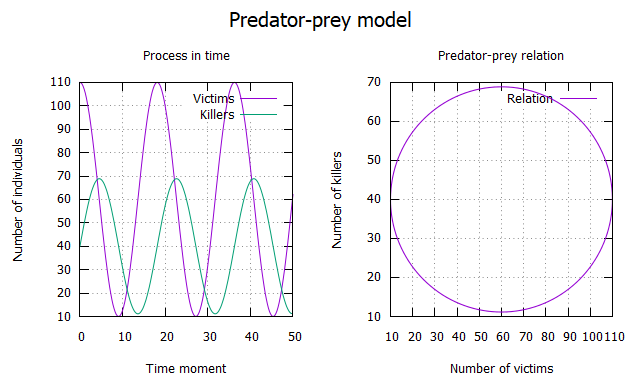
\includegraphics[width=\textwidth]{Sample1.png}
\caption{Sample input 1}
\label{fig:mpr}
\bigbreak
\centering
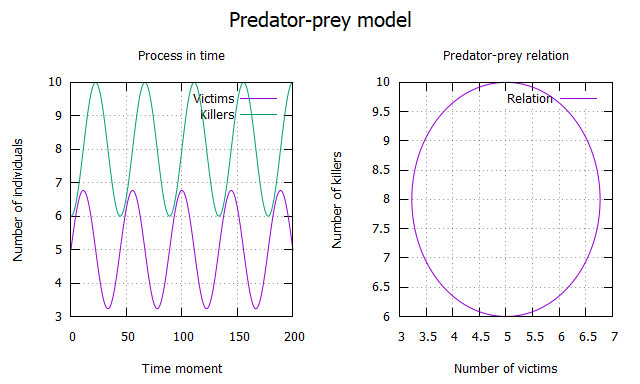
\includegraphics[width=\textwidth]{Sample2.png}
\caption{Sample input 2}
\label{fig:mpr}
\end{figure}
\bigbreak
\bigbreak
\bigbreak
\bigbreak
\bigbreak


\noindent $\textbf{2.2. Implementation of Predator-prey model.}$\\
\noindent [Online] Available:\\
\url{https://github.com/DanisAlukaev/FourthJointAssignment_LA_II}\\
The source code is located in file "main.cpp".\\
\url{https://github.com/DanisAlukaev/FourthJointAssignment_LA_II/blob/master/main.cpp}\\
\noindent Source code:

\begin{lstlisting}[language=C++, caption=Implementation of Predator-prey model]
#include <iostream>
#include <cmath>

#define INF (unsigned)!((int)0)
#ifdef WIN32
#define GNUPLOT_NAME "C:\\gnuplot\\bin\\gnuplot -persist"
#endif // WIN32

using namespace std;

/**
    Fourth Joint Assignment.
    #1.
    @author Danis Alukaev BS-19-02.
**/

/**
 * Class Matrix.
 * Represents a rectangular array of numbers arranged in rows and columns.
 */
class Matrix
{
public:
    int n, m; // dimensions of a matrix
    double **data; // the dynamic array to store elements of a matrix

    /**
    * Constructor of the class Matrix.
    * Dynamically allocates memory to store the matrix with the received number of rows and columns.
    *
    * @param rows - the number of rows of a matrix.
    * @param columns - the number of columns of a matrix.
    */
    Matrix(int rows, int columns)
    {
        n = rows; // set the number of rows
        m = columns; // set the number of columns
        // allocate memory for an array of arrays
        data = (double **) malloc(sizeof(double*) * n);
        for(int i = 0; i < n; i++)
            data[i] = (double*)malloc(sizeof(double) * m);
    }

    /**
    * Overloading " >> " operator for a class Matrix
    */
    friend istream& operator >> (istream& in, const Matrix& matrix)
    {
        for(int i = 0; i < matrix.n; i++)
            for(int j = 0; j < matrix.m; j++)
                in >> matrix.data[i][j]; // read the element with indexes i, j
        return in;
    }

    /**
    * Overloading " << " operator for a class Matrix
    */
    friend ostream& operator << (ostream& out, const Matrix& matrix)
    {
        for(int i = 0; i < matrix.n; i++)
        {
            for(int j = 0; j < matrix.m-1; j++)
                out << matrix.data[i][j] << " ";
            out << matrix.data[i][matrix.m-1] << "\n"; // print the element with indexes i, j
            // use the construction round(someNumber * 100) / 100 to round half towards one
        }
        return out;
    }

    /**
    * Overloading " = " operator for a class Matrix
    *
    * @param other - the matrix to be moved to this instance.
    * @return *this - this instance of a class Matrix.
    */
    Matrix& operator = (Matrix& other)
    {
        n = other.n; // set new dimensions
        m = other.m; // of a matrix
        data = other.data; // transfer elements to this instance of a matrix
        return *this;
    }

    /**
    * Overloading " + " operator for a class Matrix
    *
    * @param other - the matrix to be added to this instance.
    * @return *matrixN - the sum of two matrices.
    */
    Matrix& operator + (Matrix& other)
    {
        Matrix* matrixN = new Matrix(n, m); // creating new instance of the class Matrix to store the result
        for(int i = 0; i < n; i++)
            for(int j = 0; j < m; j++)
                matrixN -> data[i][j] = data[i][j] + other.data[i][j]; // store the result of an addition
        return *matrixN;
    }

    /**
    * Overloading " - " operator for a class Matrix
    *
    * @param other - the matrix to be subtracted from this instance.
    * @return *matrixN - the difference of two matrices.
    */
    Matrix& operator - (Matrix& other)
    {
        Matrix* matrixN = new Matrix(n, m); // creating new instance of the class Matrix to store the result
        for(int i = 0; i < n; i++)
            for(int j = 0; j < m; j++)
                matrixN -> data[i][j] = data[i][j] - other.data[i][j]; // store the result of a subtraction
        return *matrixN;
    }

    /**
    * Overloading " * " operator for a class Matrix
    *
    * @param other - the matrix to be multiplied by this instance.
    * @return *matrixN - the transposed matrix.
    */
    Matrix& operator * (Matrix& other)
    {
        Matrix* product = new Matrix(n, other.m); // creating new instance of the class Matrix to store the result
        for(int i = 0; i < n; i++)
            for(int j = 0; j < other.m; j++)
                product -> data[i][j] = 0; // nullify all positions of a new matrix
        for(int i = 0; i < n; i++)
            for(int j = 0; j< other.m; j++)
                for(int k = 0; k < m; k++)
                    product -> data[i][j] += data[i][k] * other.data[k][j]; // store the result of multiplication
        return *product;
    }

    /**
    * Transposition of the matrix.
    * Flips a matrix over its principal diagonal.
    *
    * @return *matrixN - the transposed matrix.
    */
    Matrix& transpose()
    {
        Matrix* matrixN = new Matrix(m, n); // creating new instance of the class Matrix to store the result
        for(int i = 0; i < m; i++)
            for(int j = 0; j < n; j++)
                matrixN -> data[i][j] = data[j][i]; // store elements of a particular row in the corresponding column
        return *matrixN;
    }

    /**
    * Destructor of the class Matrix.
    */
    ~Matrix()
    {
        for(int i = 0; i < n; i++)
            delete [] data[i];
        delete [] data;
    }
};

/**
 * Class SquareMatrix.
 * Represents the matrix with the same number of rows and columns.
 */
class SquareMatrix : public Matrix
{
public:
    /**
    * Constructor of the class SquareMatrix.
    * Creates the matrix with the same number of rows and columns.
    *
    * @param dimension - the dimension of matrix.
    */
    SquareMatrix (int dimension) : Matrix(dimension, dimension)
    {
        // creating new instance of the class Matrix with the received number of rows and columns
    }
};

/**
 * Class IdentityMatrix.
 * Represents the square matrix with ones on the main diagonal and zeros elsewhere.
 */
class IdentityMatrix : public SquareMatrix
{
public:
    /**
    * Constructor of the class IdentityMatrix.
    * Creates the square matrix with ones on the main diagonal and zeros elsewhere.
    *
    * @param dimension - the dimension of an identity matrix.
    */
    IdentityMatrix (int dimension) : SquareMatrix(dimension)
    {
        for(int i = 0; i < dimension; i++)
            for(int j = 0; j < dimension; j++)
                i == j ? data[i][j] = 1 : data [i][j] = 0; // creating the identity matrix, set the main diagonal elements to ones and fill the rest of matrix with zeroes
    }
};

/**
 * Class PermutationMatrix.
 * Represents the square matrix used to exchange two rows with received indexes of the matrix.
 */
class PermutationMatrix : public SquareMatrix
{
public:
    /**
    * Constructor of the class PermutationMatrix.
    * Creates the identity matrix with exchanged columns i1 and i2.
    *
    * @param dimension - the dimension of a permutation matrix.
    * @param i1 - the first column to be exchanged.
    * @param i2 - the second column to be exchanged
    */
    PermutationMatrix (int dimension, int i1 = 1, int i2 = 1) : SquareMatrix(dimension)
    {
        i1--; // since the number of lines of matrix in linear algebra belongs
        i2--; // to the range [1; +inf], map it to the [0; +inf]
        for(int i = 0; i < dimension; i++)
            for(int j = 0; j < dimension; j++)
                i == j ? data[i][j] = 1 : data [i][j] = 0; // creating the identity matrix, set the main diagonal elements to ones and fill the rest of matrix with zeroes
        data[i2][i2] = 0; // swap corresponding
        data[i2][i1] = 1; // elements of lines
        data[i1][i1] = 0; // to make it
        data[i1][i2] = 1; // permutation matrix
    }
};

/**
 * Class EliminationMatrix.
 * Represents the square matrix used to lead elements with received indexes of the matrix to zeroes.
 */
class EliminationMatrix : public IdentityMatrix
{
public:
    /**
    * Constructor of the class EliminationMatrix.
    * Creates the matrix that nullify the corresponding element of the received matrix.
    *
    * @param matrix - given matrix, which element [i1, i2] should be zero.
    * @param i1 - the element's line of the given matrix.
    * @param i2 - the element's column of the given matrix.
    */
    EliminationMatrix (Matrix& matrix, int i1, int i2) : IdentityMatrix(matrix.n)
    {
        i1--; // since the number of lines of matrix in linear algebra belongs
        i2--; // to the range [1; +inf], map it to the [0; +inf]
        // check the potential division by 0
        try
        {
            if (matrix.data[i2][i2] == 0)
                throw runtime_error("Division by 0");
            data[i1][i2] = - matrix.data[i1][i2] / matrix.data[i2][i2]; // calculate the coefficient that will nullify the element with received indexes
        }
        catch(runtime_error& e)
        {
            cout << e.what() << endl;
        }
    }
};

/**
 * Class ScaleMatrix.
 * Represents the matrix used to lead the diagonal matrix to the identity matrix.
 */
class ScaleMatrix : public Matrix
{
public:
    /**
    * Constructor of the class ScaleMatrix.
    * Creates the matrix which principal diagonal elements are reciprocal to corresponding elements of the received matrix.
    *
    * @param matrix - the given matrix, which principal diagonal elements should be ones.
    */
    ScaleMatrix (Matrix& matrix) : Matrix(matrix.n, matrix.n)
    {
        for(int i = 0; i < matrix.n; i++)       // treat all
            for(int j = 0; j < matrix.n; j++)   // elements of the created matrix
                data[i][j] = 0; // nullify all elements of a matrix
        for(int i = 0; i < matrix.n; i++)
            data[i][i] = 1 / matrix.data[i][i]; // set elements of the main diagonal to corresponding coefficients
    }
};

/**
 * Class AugmentedMatrix.
 * Represents matrix that can be used to perform the same elementary row operations on each of the given matrices.
 * Particularly, in this implementation it applied to find the inverse matrix.
 */
class AugmentedMatrix : public Matrix
{
public:
    /**
    * Constructor of the class AugmentedMatrix.
    * Merges the received and identity matrices by appending their columns.
    *
    * @param matrix - given matrix to be merged with identity matrix.
    */
    AugmentedMatrix(Matrix& matrix) : Matrix(matrix.n, 2 * matrix.n)
    {
        for(int i = 0; i < matrix.n; i++)
        {
            for(int j = 0; j < matrix.n; j++) // treat all columns from 0 up to n-th
                data[i][j] = matrix.data[i][j]; // copy elements of received matrix
            for(int j = matrix.n; j < 2 * matrix.n; j++) // treat all columns from n-th up to 2*n-th
                i == (j - matrix.n) ? data[i][j] = 1 : data [i][j] = 0; // set the main diagonal elements to ones and fill the rest of matrix with zeroes
        }
    }
};

/**
 * Inverses the received matrix using Gaussian Elimination approach.
 *
 * @param matrix - given matrix to be inversed.
 * @return inversed - the inversed matrix.
 */
Matrix& getInverse(Matrix& matrix)
{
    Matrix *Augmented = new AugmentedMatrix(matrix); // creating an augmented matrix
    int step = 1, swaps = 0; // the number of steps and permutations
    // nullify elements under the principal diagonal
    for(int i = 0; i < Augmented->n; i++)  // treat all rows of a matrix
    {
        // find the pivot with the maximum absolute value
        // store its index in the pivotIndex
        // store its value in the pivotValue
        int pivotIndex = i;
        double pivotValue = abs(Augmented->data[i][i]);
        for(int j = i; j < Augmented->n; j++)
        {
            if (pivotValue < abs(Augmented->data[j][i]) && ((abs(Augmented->data[j][i]) - pivotValue) >= 0.01)) // find the pivot with maximum absolute value
            {
                pivotIndex = j; // store the index of the found element
                pivotValue = abs(Augmented->data[j][i]); // store value of the found element
            }
        }
        // swap the current line with the found pivot line
        if(pivotIndex != i)
        {
            Matrix *P = new PermutationMatrix(Augmented->n, pivotIndex + 1, i + 1); // create the permutation matrix P_{pivotline+1 i+1} for a current state
            *Augmented = *P * (*Augmented); // apply the permutation matrix
            swaps++; // increment the number of permutations
        }
        for(int j = i + 1; j < Augmented->n; j++)
        {
            Matrix *E = new EliminationMatrix(*Augmented, j + 1, i + 1); // create the elimination matrix E_{j+1 i+1} for a current state
            *Augmented = *E * (*Augmented); // apply the elimination matrix
        }
    }
    // nullify elements over the principal diagonal
    for(int i = Augmented->n-1; i >= 0; i--)
    {
        for(int j = i - 1; j >= 0; j--)
        {
            Matrix *E = new EliminationMatrix(*Augmented, j + 1, i + 1); // create the elimination matrix E_{j+1 i+1} for a current state
            *Augmented = *E * (*Augmented); // apply the elimination matrix
        }
    }
    // the diagonal normalization
    Matrix *scale = new ScaleMatrix(*Augmented); // create the scale matrix for the diagonal normalization
    *Augmented = *scale * (*Augmented); // perform the diagonal normalization
    Matrix *inversed = new SquareMatrix(Augmented->n);
    // move the right part from n-th up to 2*n-th column of the augmented matrix to a created "inversed" matrix
    for(int i = 0; i < Augmented->n; i++)
        for(int j = Augmented->n; j < 2*Augmented->n; j++)
            inversed -> data[i][j - Augmented->n] = Augmented->data[i][j];
    return *inversed; // return the inversed matrix
}

/**
 * Predator-Prey Model.
 * Describes the dynamics of a biological system in which two species interact, one as a predator and the other as prey.
 * Method computes populations change through time limit T with quantization resolution N.
 *
 * @param v0 - initial number of victims.
 * @param k0 - initial number of killers.
 * @param a1 - positive real parameter describing the rate of increase in the prey population (reproduction coefficient).
 * @param b1 - positive real parameter describing the rate of decrease in the prey population (hunting coefficient).
 * @param a2 - positive real parameter describing the rate of decrease in the predator population (natural selection coefficient).
 * @param b2 - positive real parameter describing the rate of increase in the predator population (reproduction coefficient).
 * @param T - time limit.
 * @param N - number of the points of approximation.
 */
void modelPredatorPrey(int v0, int k0, double a1, double b1, double a2, double b2, int T, int N)
{

#ifdef WIN32
    FILE* pipe = _popen(GNUPLOT_NAME, "w");
#endif

    double interval =  (double) T / (double) N; // compute time interval of quantization
    Matrix* timeMoments = new Matrix(1, N + 1); // array of time moments
    Matrix* victimsPopulation = new Matrix(1, N + 1); // array of victim population size
    Matrix* killerPopulation = new Matrix(1, N + 1); // array of killer population size
    k0 -= a1 / b1; // equilibrium deduction
    v0 -= a2 / b2; // equilibrium deduction
    timeMoments -> data[0][0] = 0; // set first time moment to a 0.00
    for(int i = 1; i < N + 1; i++)
        // set the rest of time moments according to the quantization resolution
        timeMoments -> data[0][i] = timeMoments -> data[0][i - 1] + interval;
    cout << "t:\n"<< *timeMoments; // output array of time moments
    for(int i = 0; i < N + 1; i++)
    {
        double t = timeMoments -> data[0][i]; // get a time moment
        // calculate victim population size at the time moment t
        victimsPopulation -> data[0][i] = v0 * cos(sqrt(a1 * a2) * t) - k0 * sqrt(a2) * b1 / (b2 * sqrt(a1)) * sin(sqrt(a1 * a2) * t) + a2 / b2;
    }
    cout << "v:\n" << *victimsPopulation; // output array of victim population size
    for(int i = 0; i < N + 1; i++)
    {
        double t = timeMoments -> data[0][i]; // get a time moment
        // calculate killer population size at the time moment t
        killerPopulation -> data[0][i] = v0 * sqrt(a1) * b2 / (b1 * sqrt(a2)) * sin(sqrt(a1 * a2) * t) + k0 * cos(sqrt(a1 * a2) * t) + a1 / b1;
    }
    cout << "k:\n" << *killerPopulation; // output array of killer population size

    // PLOTTING AUGMENTED CHART
    if(pipe != NULL)
    {
        // chart title
        fprintf(pipe,"%s\n","set tics font ',8'");
        fprintf(pipe,"%s\n","set multiplot title 'Predator-prey model' font ',12' layout 1,2");
        // labels of axis
        fprintf(pipe, "%s\n", "set grid\nset xlabel 'Time moment' font ',8'\nset ylabel 'Number of individuals' font ',8'\n");
        // Process in time
        fprintf(pipe, "%s\n", "set title 'Process in time' font ',8'\n");
        fprintf(pipe, "%s\n", "set key font ',8'\n");
        fprintf(pipe, "%s\n", "plot '-' using 1:2 title 'Victims' with lines, '-' using 1:2 title 'Killers' with lines");
        for(int i = 0; i < N + 1; i++)
            // scatter plot of prey population size
            fprintf(pipe, "%f\t%f\n", timeMoments -> data[0][i], victimsPopulation -> data[0][i]);
        fprintf(pipe, "%s\n", "e");
        for(int i = 0; i < N + 1; i++)
            // scatter plot of predator population size
            fprintf(pipe, "%f\t%f\n", timeMoments -> data[0][i], killerPopulation -> data[0][i]);
        fprintf(pipe, "%s\n", "e");
        fflush(pipe);
        // Predator-prey relation
        fprintf(pipe, "%s\n", "set title 'Predator-prey relation' ");
        // labels of axis
        fprintf(pipe, "%s\n", "set grid\nset xlabel 'Number of victims' font ',8'\nset ylabel 'Number of killers' font ',8'\n");
        fprintf(pipe, "%s\n", "plot '-' using 1:2 title 'Relation' with lines");
        for(int i = 0; i < N + 1; i++)
            // scatter plot of relation between populations sizes
            fprintf(pipe, "%f\t%f\n", victimsPopulation -> data[0][i], killerPopulation -> data[0][i]);
        fprintf(pipe, "%s\n", "e");
        fflush(pipe);
        fprintf(pipe,"%s\n","unset multiplot");
    }

#ifdef WIN32
    _pclose(pipe);
#endif // WIN32

}

int main()
{
    cout.setf(ios::fixed); // set the decimal precision of
    cout.precision(2);     // output values
    int v0, k0, T, N; // the initial number of victims, the initial number of killers, the time limit, the number of the points of approximation resp.
    double a1, b1, a2, b2; // coefficients to compose the rate of change of victim and killer populations
    cin >> v0 >> k0 >> a1 >> b1 >> a2 >> b2 >> T >> N;
    modelPredatorPrey(v0, k0, a1, b1, a2, b2, T, N);
}

\end{lstlisting}

\end{document}
